The electronic system of the TRITIUM-Aveiro prototype consists of several PCB and is divided in two parts:
\begin{enumerate}
\item{} A PCB, which electronic scheme is shown in Figure \ref{fig:HVElectronicAveiro}, designed to power the PMTs with a negative high voltage. That consists of several high voltage power supplies, model C11152-01 from Hamamatsu Photonics \cite{PowerSupplyAveiroDataSheet}. This PCB is controled by a DAC\footnote{DAC, Digital-to-analog converter}, model MAX5500 from Maxim Integrated \cite{MAX5500DataSheet}. An Arduino Mega controls the DAC communication and is connected to a Raspberry Pi that runs the whole system.

A graphical interface, shown Figure \ref{subfig:GUI}, was developed to set up the different options in an easy way.

\begin{figure}
\centering
    \begin{subfigure}[b]{0.45\textwidth}
    \centering
    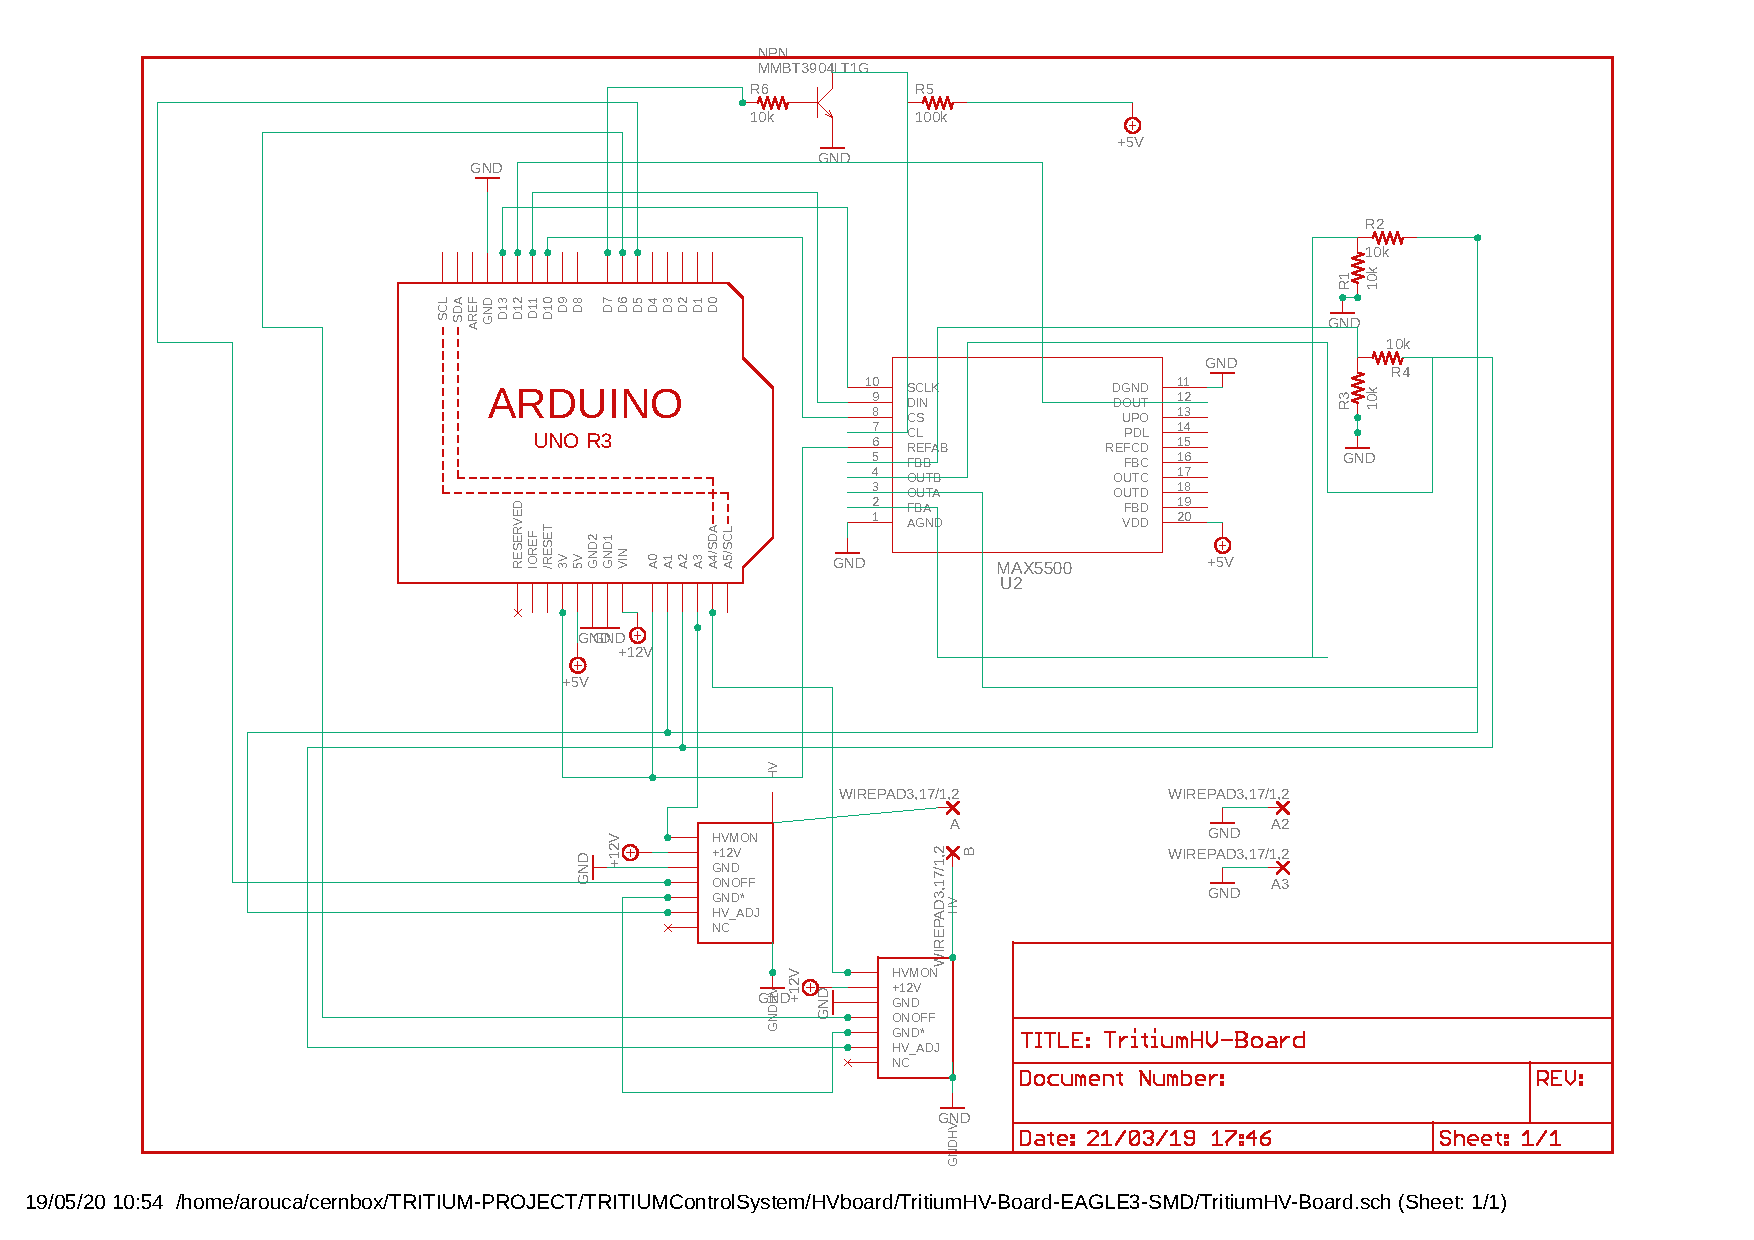
\includegraphics[width=\textwidth]{9Appendix/94AveiroElectronics/TritiumHV-Board.pdf}  
    \caption{\label{subfig:ElectronicSchemeHVBoard}}
    \end{subfigure}
    \hfill
    \begin{subfigure}[b]{0.45\textwidth}
    \centering
    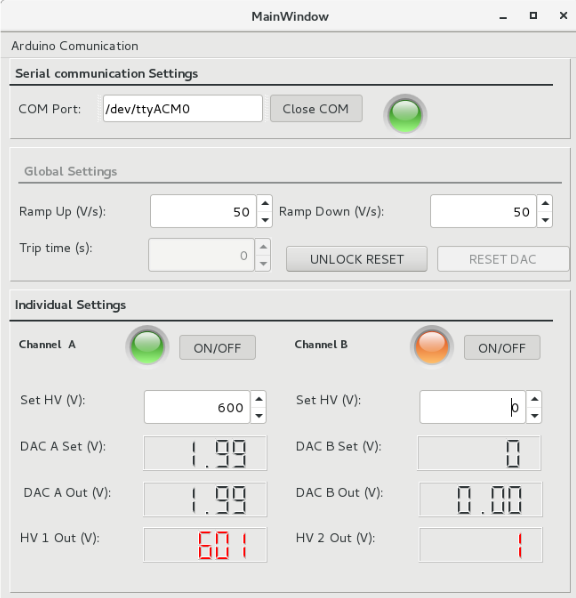
\includegraphics[width=\textwidth]{9Appendix/94AveiroElectronics/GUIHVBoard.png}  
    \caption{\label{subfig:GUI}}
    \end{subfigure}
 \caption{a) The electronic scheme of the PCB designed to power the PMTs of Aveiro prototype b) The graphical user interface developed to control the prototype.}
 \label{fig:HVElectronicAveiro}
\end{figure}

\item{} A electronic chain consisting of several PCBs that process and analyze the system signals, which electronic scheme is shown in Figure \ref{fig:ElectronicSchemCounterBoard}. This system consists of three different lines, two of them for the PMT signals of the prototype and the other for anticoincidence with an active veto.

\begin{figure}[h]
\centering
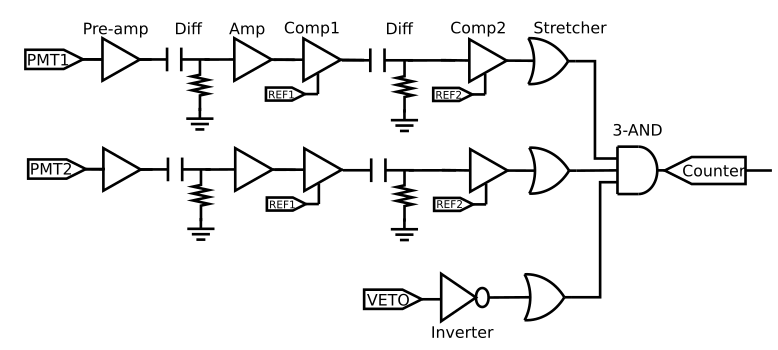
\includegraphics[scale=0.45]{9Appendix/94AveiroElectronics/ElectronicSchemeCounterBoard.png}
\caption{Electronic scheme that process and analyze the signal of the TRITIUM-Aveiro prototype. \label{fig:ElectronicSchemCounterBoard}}
\end{figure}

To test this electronic chain, a plastic scintillator of $10 \times 10 \times 1~\cm^3$ dimensions was used to simulate a veto signal. Four different vetos are being built, based on a rectangular plastic scintillators from Saint-Gobain company \cite{VetoAveiro}, of $50\times 30 \times 2~\cm^3$ dimensions. The vetos are read out by $2$" PMTs, model R2154-02 from Hamamatsu Photonics \cite{DataSheetPMTsAveiro}. The output signal of these PMTs goes into an OR stage, which output is connected to the veto line shown in Figure \ref{fig:ElectronicSchemCounterBoard}. Thus, each veto is read in anticoincidence with the TRITIUM-Aveiro prototype.

Both lines, used to process and analyze the PMT signals of the prototypes, are equal and they are used to operate in time coincidence. Each PMT signal is introduced in a preamplifier model CR111 from CREMAT Inc. \cite{CREMATPreAmplifierDataSheet}, that shapes and pre-amplifies the signal. To reduce electronic noise and signal loss, both preamplifiers are connected as close as possible to the PMTs and they are inside aluminum boxes which act as a Faraday cage.

Each preamplifier is followed by a differentiator stage, which reduces the time width of the signal and an amplifier stage, that amplifies the signal. The amplifier is model OPA656 from Texas Instruments \cite{OPA656}. 

A fast comparator, model LT111 from Linear Technology \cite{LT111}, is used to set a threshold to remove PMT signals with low amplitude (dark counts of the PMT). A MAX5500 DAC is used to configure the thresholds.

As the time width of the preamplifier output signal is too large, $200~\mu\second$, a second differentiator stage was included to reduce fake coincidences. A second comparator was added to restore a 5V square signal again.

Finally a tunable pulse stretcher based on an OR gate, model SN74AHC1 from Texas Instruments \cite{Stretcher}, is used to set the time width of each signal to $100~\nano\second$. The time coincidence windows of the system is $200~\nano\second$.

The third line consists of an inverter, which gives a $5~\volt$ signal, except when a cosmic particle is detected, in which case the signal is $0~\volt$. A stretcher is used to set the signal time width to $100~\nano\second$.

The signals from the three lines are introduced into a 3-input AND gate, model SN74LVC1G11 from Texas Instruments \cite{ANDGate}, that makes a logic level comparison. With this last stage a temporal coincidence of both PMT signals in anti-coincidence with the veto signal is obtained. The output signal of this stage is connected to a pulse counter. 

The GPIO pins of a Raspberry Pi are used to communicate with the system and configure the threshold levels. A graphical user interface, shown in Figure \ref{fig:GUIcounts}, was developed to set the counter system in an easy way.

 \begin{figure}[h]
\centering
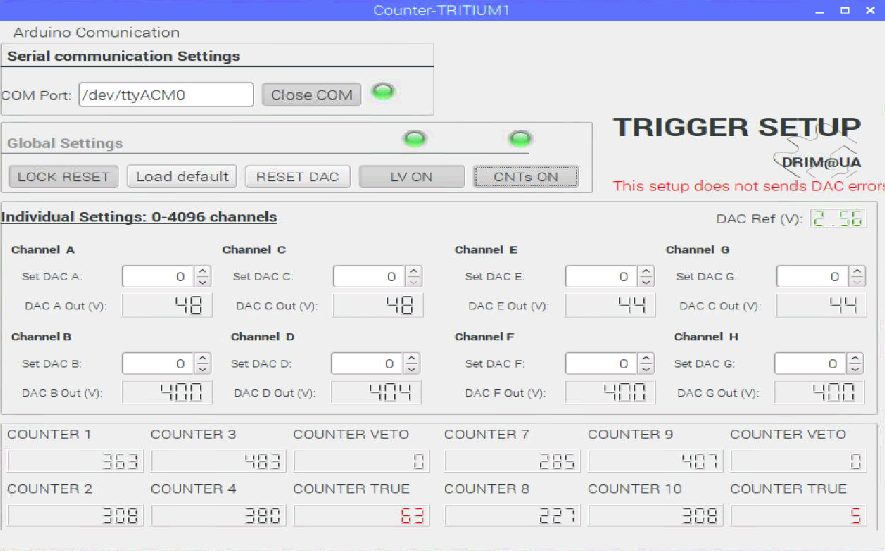
\includegraphics[scale=0.45]{9Appendix/94AveiroElectronics/CounterGUI.png}
\caption{Graphical user interface used to manage the counter system. \label{fig:GUIcounts}}
\end{figure}

Besides counting, this electronic system includes a voltage follower circuit connected to the preamplifier output signal that produces an energy spectrum for each PMT.

%It is important to note that, although this system has a graphical user interface that allows comfortable control of the system, the usual way in which it is controlled is remotely through the computer terminal.

In Figure \ref{fig:ScreenshotElectronic} screenshots for accepted an rejected events are displayed.

%In Figure \ref{fig:ScreenshotElectronic} two screenshots are shown to demostrate two different situations of this system. There, we have four different signals. The yellow and cyan signal are input signals of the AND-Gate, which come from the PMT signals of the prototype. The pink signal is the third remaining input signal of the AND-Gate, which come from the PMT signal of the veto. The last signal, green, is the output signal of the AND-Gate.

\begin{figure}
\centering
    \begin{subfigure}[b]{0.42\textwidth}
    \centering
    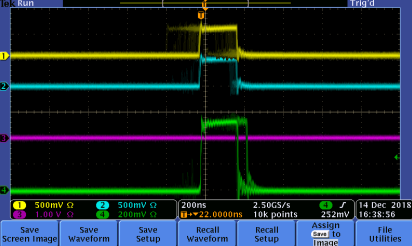
\includegraphics[width=\textwidth]{9Appendix/94AveiroElectronics/Event_accepted_Aveiro_prototype.png}  
    \caption{\label{subfig:TrueTritiumEvent}}
    \end{subfigure}
    \hfill
    \begin{subfigure}[b]{0.42\textwidth}
    \centering
    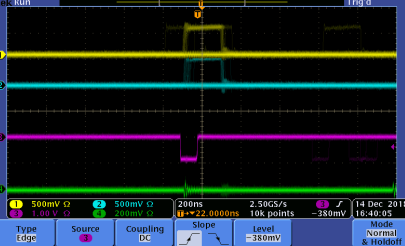
\includegraphics[width=\textwidth]{9Appendix/94AveiroElectronics/Event_rejected_Aveiro_prototype.png}  
    \caption{\label{subfig:FalseTritiumEvent}}
    \end{subfigure}
 \caption{a) Tritium event accepted as veto has not detected it. b) Background event rejected because veto has fired.}
 \label{fig:ScreenshotElectronic}
\end{figure}


%As can be seen, in Figure \ref{subfig:TrueTritiumEvent} both PMTs of the prototype have detect a time coincident event, which has not been detected for the veto, so this event is counted. In Figure \ref{subfig:FalseTritiumEvent}, a time coincidence event has been observed in the three PMTs, which means that it is a cosmic event, so this event is not counted.
\end{enumerate}